% =====================================================================
%  proposal.tex   —   WORKING COPY  (edit this one)
%
%  This is YOUR proposal. Fill in each section and delete the red
%  \begin{guidance}...\end{guidance} blocks as you go. The frozen
%  reference template (with all guidance) lives in proposal_original.tex.
%
%  Compiles to proposal.pdf  ("Working draft" on the site).
%  To hide ALL remaining guidance at once for a clean submission,
%  set \showguidance to 0 below.
% =====================================================================
\documentclass[11pt]{article}
\usepackage{forge-proposal}
\usepackage{amsmath}
\renewcommand{\showguidance}{0}   % set to 0 to hide all remaining guidance

% Centered table-header cells (border-aware): \hL for the first cell, \hC for the rest.
\newcommand{\hL}[1]{\multicolumn{1}{|c|}{\textbf{#1}}}
\newcommand{\hC}[1]{\multicolumn{1}{c|}{\textbf{#1}}}

% Giant black #TODO tag for sections awaiting real content.
\newcommand{\bigtodo}[1]{%
  \par\medskip\noindent
  \setlength{\fboxsep}{8pt}\setlength{\fboxrule}{2.5pt}%
  \noindent\fcolorbox{black}{white}{%
    \begin{minipage}{\dimexpr\linewidth-2\fboxsep-2\fboxrule\relax}
      {\fontsize{26}{30}\selectfont\bfseries\color{black}\#TODO}\\[5pt]%
      {\normalsize\bfseries\color{black} #1}
    \end{minipage}}%
  \par\medskip}

% Visible, web-style hyperlinks (blue + underline) that open in a new window/tab.
\definecolor{urlblue}{HTML}{1A5FB4}
\hypersetup{pdfnewwindow=true}
\newcommand{\urllink}[2]{\href{#1}{\textcolor{urlblue}{\underline{#2}}}}

% Hand-circled answer letter for the ethics chart (amber ring around the choice).
\usepackage{tikz}
\newcommand{\circletter}[1]{\tikz[baseline=(c.base)]{\node[draw=forgeamber,circle,line width=0.7pt,inner sep=1.2pt] (c) {#1};}}
% "Y / N / M" with N circled as the selected answer.
\newcommand{\ynmN}{Y\,/\,\circletter{N}\,/\,M}

% Persistent "Prepared by" byline placed under every section heading
% (always visible, independent of \showguidance).
\newcommand{\preparedby}{%
  \par\nobreak\vspace{-6pt}%
  {\footnotesize\itshape\color{forgemute}Prepared by Nathan Herling}%
  \par\vspace{4pt}}

% Boxed "Special Note" callout (amber rule, muted italic body).
\newcommand{\specialnote}[1]{%
  \par\medskip\noindent
  \setlength{\fboxsep}{9pt}%
  \begin{center}
  \fcolorbox{forgeamber}{white}{%
    \begin{minipage}{\dimexpr0.92\linewidth-2\fboxsep\relax}
      {\footnotesize\bfseries\color{forgeamber}SPECIAL NOTE}\\[3pt]%
      {\small\itshape\color{forgemute} #1}%
    \end{minipage}}%
  \end{center}
  \par\medskip}

\begin{document}

% ---- Masthead -------------------------------------------------------
\forgemasthead
  {\forgeexpansion}
  {Project Proposal \& Statement of Work}

\vspace{22pt}
\begin{center}
  {\Large Nathan Herling, Project Manager}\\[12pt]
  {\Large Team: Nathan Herling \textnormal{(solo capstone)}}\\[12pt]
  {\Large Faculty Advisor: Professor Ken Johns \textnormal{(UA ATLAS HEP Group)}}\\[12pt]
  {\Large Date: June 5, 2026}\\[14pt]
  {\normalsize Project documentation site:\\
   \urllink{https://n-herling-mk1.github.io/INFO_698_documentation/}%
           {n-herling-mk1.github.io/INFO\_698\_documentation}}
\end{center}

\vspace{20pt}

% ---- Skills brought to the project ----------------------------------
\begin{center}
  {\color{forgeamber}\rule{0.46\linewidth}{0.8pt}}\\[8pt]
  {\large\rmfamily\color{forgemute} Skills Brought to the Project}
\end{center}
\vspace{4pt}
{\small
This capstone draws on a cross-disciplinary foundation aligned to FORGE's three
heterogeneous reproductions and its Bayesian core:
\begin{itemize}\setlength{\itemsep}{1pt}\setlength{\parskip}{0pt}
  \item \textbf{Bayesian deep learning} --- posterior inference with Hamiltonian
        Monte Carlo and Last-Layer Laplace approximations; epistemic-vs.-aleatoric
        uncertainty quantification and calibration.
  \item \textbf{Machine-learning engineering} --- CNN, graph,
        and MLP architectures in PyTorch; training, validation, and reproducible
        experiment pipelines.
  \item \textbf{High-energy physics analysis} --- ATLAS Run~3 displaced-vertex
        long-lived-particle searches under the UA ATLAS HEP group; ROOT/CERN
        data-handling workflows.
  \item \textbf{Scientific software \& deployment} --- web dashboards, hosting, and
        continuous-integration validation across a multi-repository structure.
  \item \textbf{Cross-domain physical-science background} --- combined Physics,
        Electrical \& Computer Engineering, and Biology training, supporting
        FORGE's deliberately diverse benchmark domains.
\end{itemize}}

\clearpage

% ---- Revision History -----------------------------------------------
\section*{Revision History}
\preparedby
\renewcommand{\arraystretch}{1.25}
\begin{tabularx}{\linewidth}{|c|Y|c|}
\hline
\hL{Version} & \hC{Summary of Changes} & \hC{Date} \\ \hline
0.1 & Converted hybrid (Software + Research) template to LaTeX; title page and Executive Summary drafted & 06/01/26 \\ \hline
0.2 & Executive Summary reworked to the three-experiment elevator pitch; Sections~2/2b (user/market + literature), 3/3b (features + research deliverables), and 4 (Summer 2026 milestones + embedded Gantt) filled & 06/05/26 \\ \hline
 & & \\ \hline
\end{tabularx}

% ---- Special Note ---------------------------------------------------
\specialnote{This is a \textnormal{\textbf{hybrid proposal}} combining the Software and
Research project templates: Sections~2 and~3 each carry both a product/software track and
a research track (the \textnormal{2b} and \textnormal{3b} subsections).}

% ---- Table of Contents ----------------------------------------------
\begingroup
\renewcommand{\contentsname}{Contents}
\tableofcontents
\endgroup

\clearpage

% =====================================================================
%  1. EXECUTIVE SUMMARY
% =====================================================================
\propsec{1}{Executive Summary}
\preparedby

FORGE (Functional-posterior Observatory for Refinement and Geometric Exploration) is a web-hosted observatory built around the question every trained model hides: \emph{is its confidence earned, or has it simply run out of data?} The \emph{long term goal} is a general platform where a researcher loads their own working model, flips it from a single point estimate to a full Bayesian posterior, and steers that uncertainty in real time --- a closed-form Last-Layer Laplace Approximation (LLLA) for instant feedback, Hamiltonian Monte Carlo (HMC) for ground truth --- serving two needs from one interface: exploring whether a model has reached its \emph{epistemic limit}, and visualizing and tuning that uncertainty with Bayesian tools, with no pipeline for the user to build. The \mbox{\texttt{mk\_1}} release reported here is the \emph{proof of concept} for that vision, not the general platform itself. Rather than accept arbitrary user-supplied models, \mbox{\texttt{mk\_1}} reproduces three fixed targets drawn from deliberately different sources --- one published result, one student project, and one active research field --- preloaded by the author with documented performance, and demonstrates the Bayesian-exploration layer on those fixed reproductions. The science and the interface are real and end-to-end; what \mbox{\texttt{mk\_1}} deliberately scopes out is open-ended model ingestion, which a later release would add.

The motivation is a gap in everyday practice. A conventional network returns one number per input and reveals nothing about how much an equally valid version of the same model --- a different seed, bootstrap, or architecture --- would disagree. Bayesian inference replaces the single weight vector with a posterior $p(w \mid D)$, turning every prediction into a distribution whose width is the model's \emph{epistemic} uncertainty made visible (as distinct from \emph{aleatoric}, irreducible noise in the data).\footnote{The aleatoric/epistemic distinction follows A.\ Kendall and Y.\ Gal, ``What Uncertainties Do We Need in Bayesian Deep Learning for Computer Vision?'', NeurIPS 2017.} FORGE exposes that distinction directly in the browser and pairs it against the original deterministic baseline, lowering the barrier to interpreting model uncertainty for both specialists and reviewers. Because a posterior is computationally expensive, FORGE keeps most of the network deterministic and makes only the final layer Bayesian: the LLLA path is fast enough to resample within an interactive session, while HMC supplies the trusted reference.

The three reproductions span deliberately heterogeneous domains, to show the FORGE pattern generalizes across model classes: (1)~music-genre recognition with a convolutional network and a Bayesian classification head (GTZAN); (2)~phonon density-of-states regression with a graph network (Chen et~al., 2021); and (3)~the ATLAS Run~3 search for long-lived hidden-sector scalars via displaced muon-spectrometer vertices. Reproducing three rather than one is also a redundancy strategy: if one proves intractable on the term timeline, the proof of concept still stands on the remaining two.

% =====================================================================
%  2. USER / MARKET RESEARCH
% =====================================================================
\propsec{2}{User/Market research}
\preparedby

\propsubsub{Overall market}
FORGE sits in the uncertainty-quantification (UQ) tooling space for machine learning, which has grown alongside the adoption of Bayesian methods in the data-rich physical sciences (high-energy physics, condensed matter, materials). The existing landscape splits cleanly into five segments: deterministic ML ``playgrounds'' (no uncertainty), post-hoc posterior diagnostics shipped as libraries, probabilistic-programming frameworks, production UQ/monitoring dashboards, and interactive sampler explainers built on toy targets. None of these is a hosted, interactive instrument for asking whether a \emph{trained} model's confidence is earned. That gap --- between a code-heavy probabilistic framework and a static decision plot --- is FORGE's opening.

\propsubsub{Target users}
FORGE answers two questions with one instrument, so it serves two user types. They are not redundant: the first asks a decision question with a cost attached; the second asks an open ``how'' question. The diagnostician is the motivating problem (what makes the work worth doing); the observatory is the capability problem (what the tool literally does, and what hypotheses H1--H3, defined in Section~3b, test). Each is framed below as User\,+\,Need\,+\,Because, with the design-actionable insight in the ``Because'' clause.

\begin{table}[H]
\centering\renewcommand{\arraystretch}{1.3}
\begin{tabularx}{\linewidth}{|l|Y|}
\hline
\textbf{User 1 --- Diagnostician} & \textit{``Should I collect more data, or is this as good as it gets?''} \\ \hline
\textbf{User} & Graduate researchers in data-rich physical sciences who train their own neural-net classifiers/regressors but are \emph{not} Bayesian-ML specialists. \\ \hline
\textbf{Need} & To see whether a trained model's confidence is earned or borrowed --- whether its remaining error is epistemic (fixable with more/better data or a different architecture) or irreducible. \\ \hline
\textbf{Because} & A single point estimate hides what the model does not know, and standing up a full Bayesian pipeline from scratch is enough engineering that researchers skip it and ship overconfident models. \emph{This is exactly why FORGE preloads working baselines.} \\ \hline
\end{tabularx}
\caption{User 1 point-of-view (the motivating, diagnostic use)}
\end{table}

\begin{table}[H]
\centering\renewcommand{\arraystretch}{1.3}
\begin{tabularx}{\linewidth}{|l|Y|}
\hline
\textbf{User 2 --- Observatory} & \textit{``What is driving this uncertainty, and what happens if I change it?''} \\ \hline
\textbf{User} & Practitioners and students of Bayesian deep learning who want to understand how their modeling choices shape the posterior. \\ \hline
\textbf{Need} & An interactive instrument to reshape the posterior in real time --- turn a prior, sampler setting, likelihood, or architecture knob --- and immediately see the geometry respond. \\ \hline
\textbf{Because} & The normal Bayesian loop is slow (minutes per HMC run) and its outputs are scalars and trace plots, not geometry you can steer. \emph{This is exactly why the closed-form LLLA fast path is non-negotiable for real-time knob response (hypothesis~H3).} \\ \hline
\end{tabularx}
\caption{User 2 point-of-view (the general, exploratory capability)}
\end{table}

\propsubsub{Existing competitors}
Each comparable below overlaps FORGE on at least one axis (interactive model exploration, posterior/uncertainty visualization, sampler diagnostics, or Bayesian experimentation), paired with the line that separates it from FORGE.

\begin{table}[H]
\centering\renewcommand{\arraystretch}{1.2}
\begin{tabularx}{\linewidth}{|p{0.44\linewidth}|Y|}
\hline
\hL{Comparable} & \hC{How FORGE differs} \\ \hline
MCMC Interactive Gallery; GP-regression demo (interactive sampler/Bayesian explainers)\newline{\footnotesize\ttfamily\urllink{https://chi-feng.github.io/mcmc-demo/}{chi-feng.github.io/mcmc-demo}\newline\urllink{https://www.tmpl.fi/gp/}{tmpl.fi/gp}} & Animate samplers on \emph{fixed} 2-D targets or 1-D GP regression; FORGE samples a \emph{trained model's} weight posterior across real benchmarks and adds a deterministic-vs-Bayesian comparison. \\ \hline
TensorFlow Playground; ConvNetJS (deterministic NN sandboxes)\newline{\footnotesize\ttfamily\urllink{https://playground.tensorflow.org}{playground.tensorflow.org}\newline\urllink{https://cs.stanford.edu/people/karpathy/convnetjs/}{cs.stanford.edu/people/karpathy/convnetjs}} & Decision-boundary sandboxes with \emph{no} uncertainty; FORGE adds the epistemic layer they deliberately omit. \\ \hline
ArviZ; bayesplot; ShinyStan (post-hoc posterior diagnostics)\newline{\footnotesize\ttfamily\urllink{https://python.arviz.org/}{python.arviz.org}\newline\urllink{https://mc-stan.org/bayesplot/}{mc-stan.org/bayesplot}\newline\urllink{https://mc-stan.org/shinystan/}{mc-stan.org/shinystan}} & Plot samples you \emph{already} have; FORGE is hosted and generates and reshapes posteriors in-session. \\ \hline
PyMC; Pyro; JASP (probabilistic-programming / stats)\newline{\footnotesize\ttfamily\urllink{https://www.pymc.io/}{pymc.io}\newline\urllink{https://pyro.ai/}{pyro.ai}\newline\urllink{https://jasp-stats.org/}{jasp-stats.org}} & Code frameworks or a stats package; FORGE is the no-code ``turn a knob, watch the posterior move'' layer on top. \\ \hline
Weights \& Biases; WhyLabs; Evidently~AI (production UQ/monitoring)\newline{\footnotesize\ttfamily\urllink{https://wandb.ai/}{wandb.ai}\newline\urllink{https://whylabs.ai/}{whylabs.ai}\newline\urllink{https://www.evidentlyai.com/}{evidentlyai.com}} & Track deployed-model metrics and drift; report confidence numbers, not posteriors or Bayesian reasoning. \\ \hline
Netron (architecture viewer)\newline{\footnotesize\ttfamily\urllink{https://netron.app/}{netron.app}} & Shows structure only --- no uncertainty, posterior inference, or Bayesian reasoning. \\ \hline
\end{tabularx}
\caption{Comparable tools and how FORGE is differentiated}
\end{table}

\propsubsub{User insights and pain points}
Three pain points recur across both user types and drive the architecture directly: (i)~the engineering cost of standing up a Bayesian pipeline (HMC/NUTS, calibration, last-layer Laplace) is high enough that researchers skip it --- addressed by preloading working baselines that users inherit rather than rebuild; (ii)~the edit-code-and-wait loop is slow and its outputs are scalars and trace plots rather than steerable geometry --- addressed by the closed-form LLLA fast path that keeps the knob panel responsive, with heavy HMC reserved for ground truth; and (iii)~the elephant in the room for any trained model is whether it will \emph{generalize} and --- more pointedly --- how anyone would know, yet practitioners have no lightweight, hands-on way to interrogate it: to \emph{play} with the constraints of the model and its data and watch the epistemic limit emerge, separating confidence that is earned from confidence that is merely extrapolated, whether out of plain curiosity or as fact-finding with real-world stakes in research and industry --- addressed by FORGE's interactive exploration layer, which surfaces epistemic uncertainty (the posterior width where the data stops pinning the model down) as a visible, steerable proxy for that question rather than something a user must re-engineer from scratch. In each case the problem framing and the technical design are the same claim seen from two sides.

% ---- 2b ----
\propsec{2b}{Literature Review/Market research}
\preparedby

Because FORGE has both a software and a research element, novelty is gauged on two fronts: the comparable-tools scan above (so the build is clear of others' ground) and the ``research of research'' below --- peer-reviewed work that grounds FORGE's ingredients and sharpens where its contribution is genuinely new. A continually-updated, browsable version of this review is maintained as the \urllink{https://n-herling-mk1.github.io/INFO_698_documentation/index.html\#literature}{Literature Search} panel on the project documentation site.

\propsubsub{Methodological foundations}
Each FORGE ingredient rests on established work. Bayesian deep-learning inference: variational Bayes-by-backprop (Blundell et~al., 2015) and Monte-Carlo dropout as approximate inference (Gal \& Ghahramani, 2016). The interactive fast path: the Last-Layer Laplace Approximation and its ``Bayesian last layer'' framing (Kristiadi et~al., 2020; Daxberger et~al., 2021, \emph{laplace-torch}). The ground-truth path: Hamiltonian Monte Carlo and the No-U-Turn Sampler (Neal, 2011; Hoffman \& Gelman, 2014). The aleatoric/epistemic decomposition that motivates the whole tool: Kendall \& Gal (2017). The reproduced experiments draw on domain baselines: a graph network for phonon DOS (Chen et~al., 2021) over the DFPT phonon database (Petretto et~al., 2018), and CNN-based genre recognition (Sridhar, 2024; and the author's prior BEARDOWN work, Herling \& Attili, 2025).

\propsubsub{Closest prior art and the novelty gap}
Table~\ref{tab:priorart} collects the work nearest to FORGE's \emph{purpose}---a posterior over models used to decide where knowledge is lacking---and its \emph{interactivity}.

\begin{table}[H]
\centering\renewcommand{\arraystretch}{1.2}
\begin{tabularx}{\linewidth}{|p{0.34\linewidth}|Y|}
\hline
\hL{Reference} & \hC{Relevance to FORGE} \\ \hline
Dearden, Friedman \& Andre --- \textit{Model-Based Bayesian Exploration} (UAI 1999) & An early statement of the core FORGE logic --- a posterior over models beats a point estimate for deciding where knowledge is lacking --- but applied as an RL exploration algorithm, not a visualization tool. \\ \hline
Frazier --- \textit{A Tutorial on Bayesian Optimization} (2018) & Shares the ``visualize posterior uncertainty, decide where you're unsure'' pattern, but aimed at optimizing a function rather than diagnosing a trained model. \\ \hline
Wang, Jin, Schmitt \& Olhofer --- \textit{Recent Advances in Bayesian Optimization} (ACM CSUR 2023) & Confirms the BO field is optimization-centric; useful for positioning FORGE's model-\emph{diagnosis} purpose as distinct. \\ \hline
Gabry, Simpson, Vehtari, Betancourt \& Gelman --- \textit{Visualization in Bayesian Workflow} (JRSS-A 2019) & The methodological backbone for FORGE's plots --- but static, R-package workflow guidance, not an interactive hosted dashboard. \\ \hline
Nussbaumer, B\"ock \& Cito --- \textit{Online and Interactive Bayesian Inference Debugging} (ICSE 2026; \textit{InferLog Holmes}) & The closest prior art to FORGE's online, interactive ambition --- but an IDE debugger for PPL code aimed at \emph{fixing inference}, not a hosted multi-domain dashboard for exploring a trained model's epistemic uncertainty. \\ \hline
\end{tabularx}
\caption{Research landscape --- closest prior art}
\label{tab:priorart}
\end{table}

\propsubsub{Where FORGE is novel}
The landscape grounds each ingredient individually, but no existing system is a hosted dashboard that simultaneously (1)~preloads trained models across heterogeneous domains, (2)~toggles deterministic\,$\leftrightarrow$\,Bayesian and compares posteriors against the baseline, and (3)~reshapes posterior geometry in real time through a knob panel backed by closed-form LLLA plus heavy HMC. The combination, framed by the question \emph{``is this model's confidence earned or borrowed---has it reached its epistemic limit?''}, is the differentiated contribution.

% =====================================================================
%  3. PRODUCT FEATURES
% =====================================================================
\propsec{3}{Product Features}
\preparedby

FORGE is built in three maturity rungs of \emph{one} product, not three different products: the same application (data locked, methodology exposed) is carried up a ladder --- first proven locally (\emph{MVP --- phase~1}), then deployed (\emph{MVP --- deployed}), then optionally opened to an LLM agent (\emph{Stretch --- MCP}). The science underneath all three is identical, so the project always has a complete deliverable no matter how high the ladder is climbed. Phase~1 (features F1--F5) is everything required to demonstrate the concept locally; the deployed rung (F6) ships the same stack to a cloud host; only the MCP rung (S1) is a true stretch, and it adds no new science. All features are owned by Nathan Herling (solo capstone).

\begin{table}[H]
\centering\renewcommand{\arraystretch}{1.25}
\begin{tabularx}{\linewidth}{|c|l|Y|}
\hline
\hL{\#} & \hC{Feature} & \hC{What it does / why the user wants it} \\ \hline
\multicolumn{3}{|l|}{\textbf{MVP --- phase~1} \textnormal{(minimum feature set; local + logging)}} \\ \hline
F1 & Preloaded multi-domain baselines & Three working, documented models (genre, phonon, ATLAS) load instantly; the user inherits a baseline instead of building a pipeline. \\ \hline
F2 & Deterministic\,$\leftrightarrow$\,Bayesian toggle & Flip a trained model from a point estimate to a posterior and compare the two side by side --- the core ``is the confidence earned?'' view. \\ \hline
F3 & Real-time knob panel & Turn prior, sampler, likelihood, and architecture knobs and watch the posterior geometry respond live, backed by the closed-form LLLA fast path. \\ \hline
F4 & Posterior-geometry visualization & Credible regions, function-space spread, and the per-config posterior-$\sigma$ distribution, rendered in-browser. \\ \hline
F5 & Resource-logging layer & Per-run telemetry (memory, time, cost) that turns Phase-2 infrastructure sizing into an empirical fit rather than a guess. \\ \hline
\multicolumn{3}{|l|}{\textbf{MVP --- deployed} \textnormal{(same stack, cloud host)}} \\ \hline
F6 & Cloud deployment & The same Docker images run on a cloud host; only one environment variable changes between local and deployed. \\ \hline
\multicolumn{3}{|l|}{\textbf{Stretch --- MCP} \textnormal{(optional agent interface)}} \\ \hline
S1 & MCP server & A thin manifest advertises the compute functions as tools an LLM client (e.g.\ Claude Desktop) can call --- no new infrastructure. \\ \hline
\end{tabularx}
\caption{FORGE feature list across the three MVP rungs, all owned by N.~Herling}
\end{table}

\propsub{}{Feature F3: Real-time knob panel --- the load-bearing interactive feature}
The whole value of FORGE for User~2 depends on the knob panel feeling instant, which is why the architecture splits into two compute paths: a closed-form LLLA path on an always-on CPU for interactivity, and a heavy HMC/NUTS path on a serverless GPU for ground truth. The performance envelope is summarized in Table~\ref{tab:f3}.

\begin{table}[H]
\centering\renewcommand{\arraystretch}{1.25}
\begin{tabularx}{\linewidth}{|Y|c|c|Y|}
\hline
\hL{Parameter} & \hC{Target} & \hC{Ceiling} & \hC{Comments} \\ \hline
LLLA knob-to-update latency & $\le 1$\,s\textsuperscript{*} & $\le 3$\,s\textsuperscript{*} & Closed-form last-layer; must feel interactive \\ \hline
HMC ``ground-truth'' resample & $\sim$1\,min\textsuperscript{*} & $\le$5\,min\textsuperscript{*} & Serverless GPU, scale-to-zero; per-job, not interactive \\ \hline
Compute paths exposed & 2 & 2 & LLLA (CPU, always-on) and HMC/NUTS (GPU, on demand) \\ \hline
\end{tabularx}
\smallskip
{\footnotesize\itshape\noindent \textsuperscript{*}\,Early planning estimates, not yet profiled --- to be revisited once Phase~1 and its resource-logging layer (F5) are complete and the fitted time-vs-scale curves ($\mathrm{time}\approx f(n_{\mathrm{params}},\,n_{\mathrm{samples}},\,\ldots)$, including data size) are available. (Cold-start container spin-up and JAX/XLA compilation on the serverless GPU are not yet included in the HMC figures.)}
\caption{Feature~F3 interactive-path parameters}
\label{tab:f3}
\end{table}

\propsub{}{Feature F6: Cloud deployment (MVP --- deployed) --- hosting envelope}
Deployment must hold to a hobby-scale budget; the only component that must run continuously is one always-on CPU box, with the heavy GPU path serverless and effectively \$0 at idle. Planning estimates (as of May~2026) are in Table~\ref{tab:host}.

\begin{table}[H]
\centering\renewcommand{\arraystretch}{1.25}
\begin{tabularx}{\linewidth}{|Y|c|Y|}
\hline
\hL{Layer} & \hC{Est.\ cost/mo} & \hC{Notes} \\ \hline
Frontend (static, GitHub Pages) & $\sim$\$1 & Domain only; Pages\,+\,TLS free \\ \hline
Backend API\,+\,LLLA (Fly.io/Render) & \$10--25 & Always-on CPU box, $\sim$2\,GB RAM \\ \hline
HMC heavy jobs (Modal, serverless GPU) & $\sim$\$0 baseline & Scale-to-zero, per-second; credits cover dev \\ \hline
Database & \$0 & Stateless / explicit job-ID design; deferred \\ \hline
\multicolumn{1}{|r|}{\textbf{Target total}} & \textbf{$\sim$\$25} & \multicolumn{1}{l|}{Size of one always-on CPU box} \\ \hline
\end{tabularx}
\caption{Feature~F6 hosting-cost envelope}
\label{tab:host}
\end{table}

\propsub{}{Per-project interactive demos (the ``fidgets'')}
Each reproduction ships a hands-on demo built into its own \emph{standalone full stack} --- a local Python Flask dev server during Phase~1 --- so every project is independently runnable before Phase~2 folds them onto the shared deployed backend (these are the Phase-1 standalone sites of Section~4). All three follow one pattern: \emph{drop or tune a domain object $\rightarrow$ a scored output, an uncertainty band, and a themed visualization}, over the same \texttt{/api/predict} contract used by the \texttt{/api/eda} route. They are the user-facing realization of features F1--F4, specialized per domain; the uncertainty band is the through-line that ties them to FORGE's Bayesian spine.

\begin{table}[H]
\centering\renewcommand{\arraystretch}{1.3}
\begin{tabularx}{\linewidth}{|l|Y|Y|c|}
\hline
\hL{Project} & \hC{Interaction} & \hC{Output (scored + uncertainty + viz)} & \hC{Backing} \\ \hline
Genre & Drop an audio file & Per-genre softmax scores + audio-settings dashboard & real \\ \hline
Phonon & Build a crystal (elements\,$\rightarrow$\,formula / unit cell) & Predicted phonon DOS with a posterior ribbon; live specific heat $C_v$ and vibrational entropy on a temperature sweep & surrogate \\ \hline
ATLAS & Tune kinematic features (sliders, anchored to \texttt{eda\_stats.json}) & A point on the ABCD plane with \emph{dual} NN1/NN2 credible bands off the axes; barrel/endcap toggle; in-distribution vs extrapolation shading; LLLA live with a precomputed HMC reference & mock \\ \hline
\end{tabularx}
\caption{Per-project interactive demos. The ATLAS payoff view is the barrel region where the NN1 and NN2 bands lock together despite the measured dCor\,$\approx$\,1.79 correlation failure.}
\end{table}

\noindent Honesty caveat: only the genre demo is backed by a trained model (BEARDOWN); the phonon and ATLAS demos run against a surrogate / mock posterior until their real models land, and are labelled \emph{demo prediction} in-UI so trained and placeholder output are never confused.

% ---- 3b ----
\propsec{3b}{Research Project Deliverables}
\preparedby

\propsubsub{Hypotheses (H1--H3)}
FORGE's observatory capability rests on three testable hypotheses, each tied to a feature and checked against the HMC/NUTS ground truth:
\begin{itemize}[nosep,leftmargin=1.4em]
  \item \textbf{H1 --- visualization fidelity.} The Bayesian posterior can be rendered in-browser (credible regions, function-space spread, and the per-configuration posterior-$\sigma$ distribution; feature~F4) faithfully enough that a viewer reads the model's epistemic uncertainty correctly rather than an artifact of the display. \emph{Tested by} comparing the rendered credible regions and their coverage against the ground-truth posterior.
  \item \textbf{H2 --- sampler correctness and efficiency.} The closed-form LLLA fast path agrees with the ground-truth HMC/NUTS posterior within tolerance (correctness) while staying fast enough to resample inside an interactive session (efficiency; the F3 latency envelope). \emph{Tested by} LLLA-vs-HMC agreement on posterior moments and interval coverage, alongside the measured knob-to-update latency.
  \item \textbf{H3 --- hyperparameter\,$\rightarrow$\,posterior geometry (the keystone).} Turning the prior, sampler, likelihood, and architecture knobs produces systematic, interpretable, \emph{steerable} changes in posterior geometry --- the mapping is legible enough that a user can deliberately steer uncertainty in real time. This is the project's central claim and the reason the LLLA fast path is non-negotiable. \emph{Tested by} demonstrating reproducible, interpretable posterior-geometry responses to knob changes across the three reproductions.
\end{itemize}

\propsubsub{Final presentation format}
The project culminates in (i)~a written report with introduction, methods, and results sections and at least five peer-reviewed citations, carrying at least two informative graphics (the deterministic-vs-Bayesian comparison and the fitted resource-cost curves); (ii)~a poster and live demo for the project presentation; and (iii)~the deployed FORGE site plus three public GitHub repositories (documentation, experiments, software), tagged \texttt{v1.0} at freeze.

\propsubsub{What analysis is being run}
Three reproductions, each driven to a functional ground-truth result before the next begins, then extended with Bayesian inference:
\begin{itemize}[nosep,leftmargin=1.4em]
  \item \textbf{Genre recognition} --- a CNN with a Bayesian classification head over GTZAN (spectrogram + engineered-feature encoders).
  \item \textbf{Phonon DOS} --- a graph network with a Bayesian last-layer head over the 51-point DOS output; the published baseline gives point predictions only, so calibrated credible intervals are FORGE's added contribution.
  \item \textbf{ATLAS LLP} --- a deterministic MLP discriminating signal (HSS\,$\rightarrow$\,LLP) from QCD background, extended with HMC over the output layer.
\end{itemize}
Across all three, the analysis is posterior inference via the closed-form LLLA fast path and ground-truth HMC/NUTS, evaluated for calibration coverage in addition to raw accuracy.

Each reproduction ships between one and three trained models to the FORGE site, so the platform can showcase \emph{differences between models}, not merely a single model's uncertainty:
\begin{itemize}[nosep,leftmargin=1.4em]
  \item \textbf{(1)~Faithful reproduction (required).} A model reproduced to the source work's reported configuration and performance --- the fidelity anchor, present for every experiment.
  \item \textbf{(2)~Author-optimized variant (target).} A model selected and tuned with the reliability-aware Bayesian metric of Appendix~C, which scores candidates on accuracy, posterior uncertainty, and cross-validation stability rather than accuracy alone --- the model on which FORGE's epistemic-selection idea is exercised in practice.
  \item \textbf{(3)~Data-permitting variants (stretch).} Where the dataset supports it, additional flavors of~(2) that vary the input regime --- e.g.\ for genre recognition, parallel 30-second and 3-second-clip models whose posteriors can be compared head-to-head.
\end{itemize}
Model~(1) is a hard deliverable for all three reproductions; (2) is the goal wherever the term timeline allows; (3) is opportunistic.

\propsubsub{What accuracy is expected}
Each reproduction commits up front to targets drawn from its source work --- FORGE's ``empirical contract'' for declaring a baseline reproduced. Calibration coverage is the additional contribution layered on top. These targets govern the faithful reproduction (model~1); the author-optimized variant (model~2) is judged instead by the reliability-aware composite of Appendix~C, not by beating the fidelity target.

\begin{table}[H]
\centering\renewcommand{\arraystretch}{1.25}
\renewcommand{\tabularxcolumn}[1]{m{#1}}% vertically center all cells in this table
\begin{tabularx}{\linewidth}{|>{\raggedright\arraybackslash}m{0.18\linewidth}|Y|}
\hline
\hL{Experiment} & \hC{Reproduction target} \\ \hline
Genre recognition & Best-config validation accuracy $\ge 0.75$ (cfg\_14: 0.766); sweep mean $\approx 0.72$; per-genre F1 in $0.46$--$0.89$ (BEARDOWN, Herling \& Attili 2025). \\ \hline
Phonon DOS & $\ge 70\%$ of test materials within $10\%$ relative error on the average phonon frequency; per-element DOS MSE $10^{-3}$--$10^{-1}$ (Chen et~al.\ 2021). \\ \hline
ATLAS LLP &
\begin{itemize}[nosep,leftmargin=1.2em,topsep=2pt]
  \item \textbf{Reproduce the baseline (Schott 2024\footnotemark):} matched two-hidden-layer $128$--$128$ MLPs --- ReLU hidden, sigmoid output; binary-crossentropy loss, Adam; 10 epochs, batch 32; 75/25 split with signal and background reweighted to equal summed weight; uncorrelated feature sets (NN1 isolation/activity, NN2 spatial distribution).
  \item \textbf{Acceptance:} NN1 train/test ROC--AUC agreement, barrel and endcap (overtraining check); NN1/NN2 plane Pearson correlation $\approx 1\%$ (barrel), $2\%$ (endcap), preserving the ABCD axis-independence requirement; A-region thresholds NN1,\,NN2 $>0.5$ (barrel), $>0.8$ (endcap).
  \item \textbf{NN2 gap:} no standalone ROC/AUC in the source --- only the joint-plane correlation constrains its discriminating power.
  \item \textbf{Extend (new):} beyond the faithful reproduction, add architectures from recent results (Herling, Mar.\ 2026), selected with the Appendix~C reliability-aware metric --- supplying the model~(2)/(3) variants and a standalone calibrated NN2 the baseline lacks.
\end{itemize} \\ \hline
\end{tabularx}
\caption{Per-experiment reproduction targets}
\end{table}
\footnotetext{M.~L.\ Schott, \textit{Search for Long-Lived Particles Decaying into Displaced Hadronic Jets in the Muon Spectrometer in $pp$ Collisions at $\sqrt{s}=13$~TeV with the ATLAS Detector}, Ph.D.\ dissertation, Department of Physics, The University of Arizona, 2024.}

\propsubsub{What if the analysis doesn't work}
A null result is acceptable and, in this project, often \emph{informative}: a model shown to sit at its epistemic limit is exactly the diagnostic FORGE exists to surface. Risk is further managed by redundancy --- three reproductions mean the platform still demonstrates the concept if one proves intractable --- and by a dedicated three-week risk-management window (Weeks~8--10) that absorbs slippage from Phase~1 or Phase~2. The descope order is fixed: drop the MCP stretch (S1) first, then trim the depth of the Bayesian/visualization refinements; the three baseline reproductions (the guaranteed floor) and the write-up are never cut, because they carry the deliverable.

\propsubsub{What if the data isn't available}
There is no scraping dependency. All three datasets are public or already in hand: GTZAN (genre); the DFPT phonon database via the Materials Project (phonon, Petretto et~al.\ 2018); and the ATLAS reproduction inputs from the author's prior thesis work and Monte-Carlo samples. The C0--C3 calibration tiers are analytic, so their ground truth is always available for the CI scoring path regardless of external data.

% =====================================================================
%  4. PROJECT TIMELINE & GANTT CHART
% =====================================================================
\propsec{4}{Project Timeline \& Gantt Chart}
\preparedby

The thirteen-week schedule (single contributor) is anchored at Week~0 = May~18, 2026, and is organized around the three MVP phases. Weeks~0--3 cover intro, planning, and setup (proposal mk\_1 at W2, full proposal at W3). \textbf{Phase~1} (Weeks~4--6) stands up the three reproductions one per week --- genre recognition (W4), phonon DOS (W5), and the ATLAS LLP search (W6) --- each as a functional standalone site driven to ground truth, with the minimum Bayesian options (LLLA + HMC), a local dashboard, and built-in compute-recording metrics; having all three functional by Week~6 is the guaranteed ``floor'' deliverable. \textbf{Phase~2} (Weeks~7--9) ties the three repositories into one deployed FORGE website, moves off localhost to external hosting, tests and debugs, and finalizes the Bayesian-tuning and dashboard decisions; the write-up begins in Week~9. \textbf{Phase~3 / stretch} (Week~10) locks the MVP and freezes the repositories, attempting the MCP stretch only if time allows. A dedicated \textbf{three-week risk-management window (Weeks~8--10)} absorbs slippage before the write-up (W11) and the short hand-in week (W12). Table~\ref{tab:milestones} lists the dated milestones; Figure~\ref{fig:gantt} is the corresponding Gantt.

\begin{longtable}{|p{10.4cm}|c|}
\hline
\hL{Milestone} & \hC{Date} \\ \hline
\endfirsthead
\hline
\hL{Milestone} & \hC{Date} \\ \hline
\endhead
Course orientation; three repositories bootstrapped \textnormal{(course)} & 5/22/26 \\ \hline
Project Proposal mk\_1 submitted \textnormal{(course)} & 6/5/26 \\ \hline
Full proposal; timeline + Gantt locked \textnormal{(course)} & 6/12/26 \\ \hline
Music Genre standalone site functional (ground truth) & 6/19/26 \\ \hline
Phonon DOS standalone site functional (ground truth) & 6/26/26 \\ \hline
\textbf{ATLAS LLP standalone site functional --- all three at ground truth (floor)} & 7/3/26 \\ \hline
Repos integrated into FORGE website; deployed to external hosting (Phase~2) & 7/17/26 \\ \hline
Software feature-frozen; write-up begun & 7/24/26 \\ \hline
MVP + repos locked; MCP stretch attempted if time \textnormal{(risk window W8--W10)} & 7/31/26 \\ \hline
Write-up complete; deliverables locked & 8/7/26 \\ \hline
Final submission \& project presentation; repo freeze + v1.0 tag \textnormal{(course)} & 8/12/26 \\ \hline
\caption{Milestone Schedule (Summer 2026)}
\label{tab:milestones}
\end{longtable}

\noindent The Gantt chart in Figure~\ref{fig:gantt} mirrors this schedule. Its source of truth is two hand-edited files in the documentation repository: \texttt{data/gantt.json} drives the bars (per-task phase, start/end week, and status) and encodes the shaded risk-management window via a \texttt{windows} entry, while \texttt{data/weekly\_todos.json} holds each week's progress report --- three lists per week (\emph{planned}, \emph{refactored}, \emph{accomplished}) keyed to weeks W0--W12 --- that populate the interactive Gantt's clickable week-detail panel on the project site and double as the weekly status update. A live version (clickable per-week detail, downloadable PNG) is maintained at the documentation site linked below.

\begin{figure}[H]
\centering
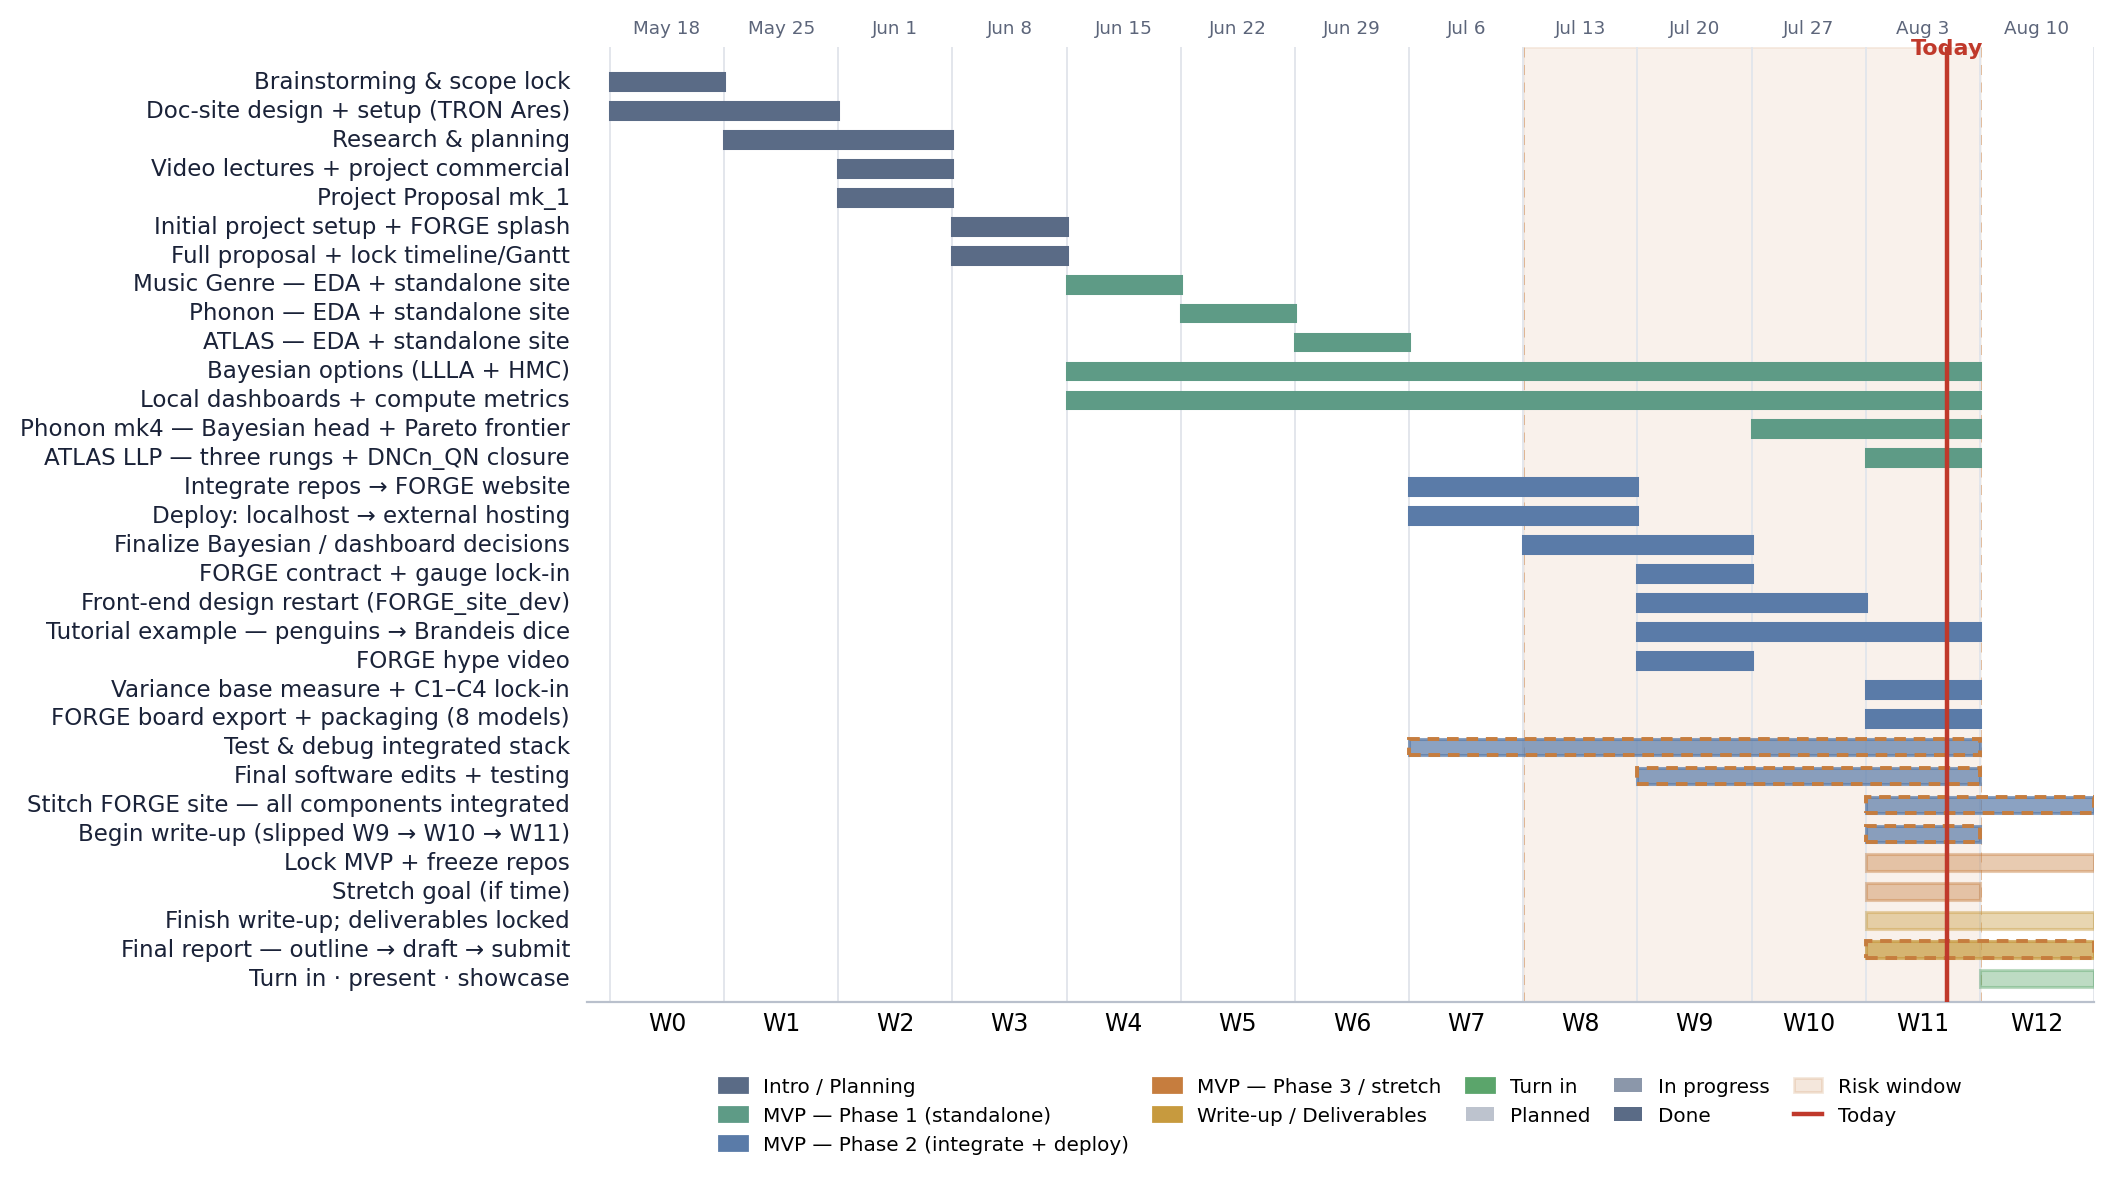
\includegraphics[width=\linewidth]{gantt_chart.png}
\caption{FORGE project Gantt (snapshot). Bars span the weeks each task is active and are colored by phase (Intro/Planning, MVP Phase~1--3, Write-up/Deliverables); fill density encodes status (planned / in progress / done); the shaded band marks the risk-management window (W8--W10) and the vertical line marks ``today''. Live version: \href{https://n-herling-mk1.github.io/INFO_698_documentation/index.html\#gantt}{n-herling-mk1.github.io/INFO\_698\_documentation \#gantt}.}
\label{fig:gantt}
\end{figure}

% =====================================================================
%  5. ETHICS
% =====================================================================
\propsec{5}{Ethics}
\preparedby
\begin{guidance}
Data ethics is a key consideration in any product we create. Include a completed ethics chart (see examples on D2L). For each question, answer Y / N / M (Yes / No / Maybe) for general use and for the data-breach scenario.
\end{guidance}

\noindent\textbf{ATLAS data note.} Whether the ATLAS/CERN detector data underlying the LLP reproduction may be released publicly is still being vetted under the collaboration's data-access and publication policy (with advisor input). If public release is not permitted, the fallback is to keep the data private and release only the model and methodology --- which is sufficient for the FORGE demonstration, since the platform's contribution is the reliability-aware methodology rather than the raw detector inputs.

\renewcommand{\arraystretch}{1.2}
\begin{longtable}{|c|p{9.5cm}|c|c|}
\hline
\hL{\#} & \hC{Question} & \hC{Generally} & \hC{Data Breach} \\ \hline
\endfirsthead
\hline
\hL{\#} & \hC{Question} & \hC{Generally} & \hC{Data Breach} \\ \hline
\endhead
1 & Could a user sell drugs or other illegal items on your platform? & \ynmN & \ynmN \\ \hline
2 & Could a user of your platform engage in sex trafficking? & \ynmN & \ynmN \\ \hline
3 & Could a user sell class notes or cheat on their homework on your platform? & \ynmN & \ynmN \\ \hline
4 & Could a stalker use your project to find someone? & \ynmN & \ynmN \\ \hline
5 & Could your app be used to spy on or track individuals? & \ynmN & \ynmN \\ \hline
6 & Could your app/software access the camera or microphone and record things without users being aware? & \ynmN & \ynmN \\ \hline
7 & If someone uses your platform, could they be re-traumatized or have their mental health impacted in some way? & \ynmN & \ynmN \\ \hline
8 & Could your algorithm promote material that would traumatize or upset individuals? & \ynmN & \ynmN \\ \hline
9 & Would your users be upset if the data you collect was given to someone else? & \ynmN & \ynmN \\ \hline
10 & Could a data leak potentially lead to identity theft? & \ynmN & \ynmN \\ \hline
11 & If your site was hacked, would users potentially lose their job, spouse, or family? & \ynmN & \ynmN \\ \hline
12 & Should there be an age limitation on your product? & \ynmN & \ynmN \\ \hline
13 & Could someone use your product to find, contact, and potentially commit elder abuse? & \ynmN & \ynmN \\ \hline
14 & If the data on your platform was breached, could it be used to blackmail the users? & \ynmN & \ynmN \\ \hline
15 & Does the existence of your project imply that a particular racial group, gender, religion, or other protected category is inherently bad, gross, or unwanted? & \ynmN & \ynmN \\ \hline
16 & Could your product be used to commit hate crimes against a specific group? & \ynmN & \ynmN \\ \hline
17 & Does the primary content of your game or algorithm focus on something considered deeply unethical? & \ynmN & \ynmN \\ \hline
18 & Does your game or software contain race, gender, or other stereotypes? & \ynmN & \ynmN \\ \hline
19 & Could users of your app scam other individuals? & \ynmN & \ynmN \\ \hline
20 & Is your particular algorithm biased toward predicting correctly only for one race, gender, or other group? & \ynmN & \ynmN \\ \hline
21 & Are the users of your project aware of how their data will be used? & \ynmN & \ynmN \\ \hline
22 & What are the possible misinterpretations of your results? & \ynmN & \ynmN \\ \hline
23 & Does the use or purchase of your data potentially contribute to a dangerous group or regime? & \ynmN & \ynmN \\ \hline
24 & Could your virtual reality environment cause injury to the user? & \ynmN & \ynmN \\ \hline
25 & Are your study participants or game players aware that their data will be collected and used? & \ynmN & \ynmN \\ \hline
26 & Does your game or app contain addictive design elements without benefit to the user? & \ynmN & \ynmN \\ \hline
27 & Does your survey contain an aspect of compulsion or unusually large incentive that would command users to take it even to their detriment? & \ynmN & \ynmN \\ \hline
28 & Could your research outcomes harm an individual or entity? & \ynmN & \ynmN \\ \hline
\caption{Data Ethics Chart}
\end{longtable}

% =====================================================================
%  6. APPROVALS
% =====================================================================
\propsec{6}{Approvals}
\preparedby
\begin{guidance}
The project proposal needs the approval of everyone to move forward. If approval is denied, rework the proposal and begin the approval cycle again. Consult the faculty advisor often. After the faculty advisor and team are comfortable with the SOW, only then should it go to the sponsor.

Type the names in the ``Approver Name'' column; written signatures only in the ``Signature'' and ``Date'' columns. Give advisors and sponsors at least 3 business days of lead time. Your instructor signs after grading, if the document passes. Keep the language below.
\end{guidance}

\noindent The signatures of the people below indicate an understanding of the purpose and content of this document by those signing it. By signing this document, you indicate that you approve of the proposed project outlined in this Statement of Work, the division of work, the Ground Rules, and that the next steps may be taken to create a Product Specification and proceed with the project.

\smallskip
\noindent This Statement of Work is self-contained: it is not derived from a separate Product Requirements Document (PRD) and is the governing specification for the FORGE capstone. Any subsequent change is tracked through the Revision History above.

\medskip
\renewcommand{\arraystretch}{1.6}
\begin{tabularx}{\linewidth}{|>{\centering\arraybackslash}p{0.24\linewidth}|c|>{\centering\arraybackslash}X|>{\centering\arraybackslash}p{0.13\linewidth}|}
\hline
\hL{Approver Name} & \hC{Title} & \hC{Signature} & \hC{Date} \\ \hline
Nathan Herling & Project Lead & & \\ \hline
Ken Johns, PhD & Faculty Advisor & & \\ \hline
Nitika Sharma, PhD & Instructor & & \\ \hline
\end{tabularx}

\begin{guidance}
Before you submit to advisor/sponsor for review: refresh the table of contents; verify every table and figure has a number and caption with at least one introductory sentence; clean up white space and page breaks; make sure the revision block is correct.

Before you submit for grading, update the author table below. It need not be 100\% accurate but should give the instructor a good idea of how much each person contributed. For tables and diagrams just put n/a for the word count.
\end{guidance}

\medskip
\renewcommand{\arraystretch}{1.4}
\begin{tabularx}{\linewidth}{|Y|l|c|}
\hline
\hL{Section} & \hC{Author} & \hC{Word Count} \\ \hline
1. Executive Summary & Nathan Herling & $\sim$420 \\ \hline
2 / 2b. User/Market \& Literature Review & Nathan Herling & $\sim$1330 \\ \hline
3 / 3b. Product Features \& Research Deliverables & Nathan Herling & $\sim$1240 \\ \hline
4. Timeline \& Gantt (incl.\ tables/figure) & Nathan Herling & n/a \\ \hline
\end{tabularx}

% =====================================================================
%  7. APPENDIX
% =====================================================================
\propsec{7}{Appendix}
\preparedby

\propsub{A.}{Advisor Engagement}

\propsubsub{Project Team Responsibilities}
\begin{itemize}[leftmargin=1.4em]
  \item The Project Manager will set up and facilitate a weekly call/meeting with the Faculty Advisor. The Project Team will provide weekly status updates including upcoming deliverables, critical issues, and any adjustments to the Project Plan.
  \item Documents will be provided to the Faculty Advisor with adequate time for review and signature, with a minimum review time of 3 days prior to the document due date.
  \item Design files will be provided to the Faculty Advisor as requested in an agreed format.
  \item Support requirements will be clearly requested with the dates required and adequate time for fulfillment.
  \item Modification requests to the Project Plan by the Faculty Advisor will be reviewed and agreed to within 1 week of the request.
\end{itemize}

\propsubsub{Faculty Advisor Responsibilities}
\begin{itemize}[leftmargin=1.4em]
  \item The Faculty Advisor will provide knowledge and expertise to help the group stretch their skills.
  \item The Faculty Advisor will participate in a weekly or bi-weekly call/meeting to review status, upcoming deliverables, priorities, issues, and progress to the agreed Project Plan.
  \item The Faculty Advisor will provide document review, feedback, and approval (or rejection, or approval with contingencies) with adequate time for the team to meet course due dates.
  \item The Faculty Advisor will provide feedback on support requirements, including guidance on design decisions, design files, test plans, test procedures, and test results.
  \item The Faculty Advisor shall provide technical advice and guidance, answering inquiries approximately 1 hour per week.
  \item Modifications to the Project Plan by the Project Team will be resolved and documented within 1 week of the request.
  \item Grade the finalized project using a skill-based rubric.
  \item Attend the project presentation.
\end{itemize}

\propsub{B.}{Ground Rules}
\begin{guidance}
How the team will conduct the business of completing this project. Each team member must sign the Approvals section indicating their acknowledgement of these Ground Rules. Do not remove items from this list, but you may add items.
\end{guidance}

\noindent As a team and as individual team members, we agree to:
\begin{itemize}[leftmargin=1.4em]
  \item \textbf{Stay focused on our objectives and goals.} Each time the team meets, we will clearly define our objectives and desired outcomes at the beginning of the meeting, and politely remind team members if we are getting off track.
  \item \textbf{``Sidebar'' issues that are relevant but not consistent with the immediate objectives.} Create a ``sidebar'' where off-topic but important matters can be listed and discussed later.
  \item \textbf{Listen when others are speaking.} We will listen and consider others' input before adding our own comments.
  \item \textbf{All viewpoints will have an opportunity to be heard.} We will make an effort to get each team member's viewpoint and ensure no one dominates the discussion.
  \item \textbf{Differences of opinion will be discussed respectfully.} We will identify areas of agreement before assessing disagreement, weigh the merits of different opinions, and agree on a process for choosing a direction. All team members will respect and follow the decision.
  \item \textbf{Look for the good points in new ideas.} We will explore the value in each idea as we assess and select our path forward.
  \item \textbf{Focus on the future, not the past.} We will use past experience to inform decisions but focus the discussion on future objectives; blame is counterproductive.
  \item \textbf{Agree upon specific action items and next steps.} At the end of each meeting we will summarize and agree on specific next steps, action items, and assignments.
  \item \textbf{Accountability.} Each member is responsible for their individual assignments and contribution to the team objectives. We will honor our responsibilities and not let our team members down.
\end{itemize}

\propsub{C.}{Exploratory Reliability-Aware Selection Metrics}
\noindent\textbf{Source.} The code and the full BEARDOWN report --- including Figures~6--7 and the metric tables of its Appendix~B --- are public: \urllink{https://github.com/N-Herling-Mk1/INFO_510_Fa25_Final_Proj}{BEARDOWN repository} and \urllink{https://github.com/N-Herling-Mk1/INFO_510_Fa25_Final_Proj/blob/main/_docs/INFO_510_FA_25_Final_Project_Group_7.pdf}{BEARDOWN report (PDF)}.

\smallskip
This appendix collects an author-developed, \emph{exploratory} suite of selection metrics: proof-of-concept rather than established canon, but each resting on a stated hypothesis with initial empirical support. They are used only to \emph{steer model selection during hyperparameter sweeps}, never to report results --- Section~3b's numbers use standard metrics (accuracy, precision/recall/F1, ROC--AUC, ECE) and stay comparable to published baselines, while the selection criterion is free to be more opinionated. The premise: accuracy alone is a poor sweep objective when the target is a \emph{reliable} model, since a configuration can top validation accuracy while being unstable across folds or badly miscalibrated --- exactly the failure mode FORGE exists to expose.

\smallskip
\noindent\textbf{Robust Ranking Metric (RRM) --- the anchor.} For a configuration scored under $k$-fold cross-validation, form a three-axis penalty vector measuring inaccuracy, instability, and posterior uncertainty, and aggregate by Euclidean distance from the ideal $\mathbf{v}=\mathbf{0}$:
\[
  \mathbf{v}=\Bigl(\,1-\bar{a},\ \ \frac{\sigma_{\mathrm{fold}}}{\sigma_{\max}},\ \ \frac{U_{\mathrm{mean}}}{U_{\max}}\,\Bigr),
  \qquad
  \mathrm{RRM} = 1-\lVert\mathbf{v}\rVert_2 .
\]
Here $\bar{a}$ is the mean fold accuracy, $\sigma_{\mathrm{fold}}$ the standard deviation of the per-fold accuracies, and $U_{\mathrm{mean}}=\operatorname{mean}\sqrt{\operatorname{diag}\Sigma}$ the mean posterior standard deviation of the Bayesian head. Selection \emph{maximizes} RRM; it reaches $1$ only for a perfectly accurate, stable, zero-uncertainty model, so nothing can win on accuracy alone while unstable or diffuse. The stability and uncertainty axes are normalized by running sweep maxima ($\sigma_{\max},U_{\max}$, floored at $10^{-8}$) onto a common $[0,1]$ scale; the uncertainty axis is the same posterior signal FORGE visualizes, here turned into an objective. Locked and run in BEARDOWN over two 20-configuration, 3-fold sweeps (\texttt{mk5l}/\texttt{mk5m}).

\smallskip
\noindent\textbf{Preliminary evidence --- non-redundancy.} RRM earns its place only if it carries information the standard metrics do not. In BEARDOWN (Herling \& Attili, 2025, Figs.~6--7) RRM correlated with accuracy at only $r\approx0.62$ ($R^2\approx0.38$, and partly by construction, since accuracy is one of its components), negatively with the uncertainty axes ($r\approx-0.33,\,-0.37$), and was statistically indistinguishable from uncorrelated with an \emph{external} diagnostic not built into it --- off-diagonal confusion noise ($r\approx0.26$, $p\approx0.26$). No single existing metric reproduces its ranking: several high-accuracy configurations scored low on RRM, and some lower-accuracy ones ranked higher. The honest reading is \emph{non-redundant}, not orthogonal --- RRM occupies a distinct direction in metric space rather than re-expressing accuracy. Because Pearson $r$ captures only \emph{linear} association while RRM is a nonlinear (norm) statistic, the planned next diagnostic is distance correlation (dCor, and partial-dCor controlling for the shared accuracy term), which measures dependence without the linearity assumption; the present correlations are exploratory, small-$n$ estimates.

\smallskip
\noindent\textbf{Open question --- the weighting.} Collapsing three heterogeneous axes into one scalar requires a relative weight per axis, $\mathbf{w}=(w_0,w_1,w_2)$, and a fixed choice is both arbitrary and game-able. Because only \emph{relative} emphasis affects the ranking, the weights are normalized to sum to one --- i.e.\ constrained to the probability simplex $\Delta^{2}=\{\mathbf{w}:w_i\ge 0,\ \sum_i w_i=1\}$, the triangle whose three corners place all weight on a single axis and whose centroid weights the three equally:
\[
  \mathrm{RRM}_{\mathbf{w}} = 1-\sqrt{\textstyle\sum_i w_i\,v_i^{2}},
  \qquad \mathbf{w}\in\Delta^{2}.
\]
The locked metric is the equal-weight case --- the centroid $\mathbf{w}=(\tfrac13,\tfrac13,\tfrac13)$ --- which ranks configurations identically to $1-\lVert\mathbf{v}\rVert_2$. Rather than fix $\mathbf{w}$, the intended treatment \emph{samples} it: each weighting is drawn from a Dirichlet distribution $\mathbf{w}\sim\mathrm{Dir}(\boldsymbol{\alpha})$, which lands on $\Delta^{2}$ by construction, so every draw is a valid weighting with no grid or renormalization step. The concentration $\boldsymbol{\alpha}$ sets the coverage pattern: $\boldsymbol{\alpha}=(1,1,1)$ samples the triangle uniformly (no prior preference); large $\boldsymbol{\alpha}$ concentrates draws near the equal-weight centroid (a local sensitivity check); small $\boldsymbol{\alpha}$ pushes them toward the corners (single-axis stress tests). The selection's sensitivity to $\mathbf{w}$ is then reported. This turns ``how independent is RRM of accuracy?'' from a fixed property into a tunable one: the weight slides the metric between an accuracy proxy (mass on $v_0$) and pure reliability (mass off it), letting one choose the weighting that maximizes added information while still selecting good models.

\smallskip
\noindent\textbf{Roadmap.} Beyond RRM the suite includes weight-free global comparisons (rank-aggregation and Pareto-front selection over accuracy and Bayesian reliability; BEARDOWN App.~B) and two candidate fourth axes $v_3$: a false-positive/false-negative--structure term, and, for the ATLAS reproduction specifically, an ABCD background-closure-quality term. All are exploratory and not claims of the main proposal. The configuration this procedure selects is the author-optimized variant (model~2) delivered for each reproduction in Section~3b.

\end{document}
